\chapter{Kalman filtering} \label{chap:kalman}

\section{Linear filtering}
Idea is that the system can be described with set of states that evolve in time. There can be various number of states and all of them are grouped together in the state vector. Navigation system could, for instance, group together position coordinates and orientation angles in the state vector. If the system is considered as discrete, transition from one discrete value of the state vector to the next one, is described with the function $f$ called process model, equation ~\ref{eq:state-transition}, where the current state, $x(k+1)$, is calculated using the process model with prevoius state ($x(k)$), current input ($u(k+1)$) and process noise ($v(k+1)$) as arguments. In other words, model mathematically describes how the state changes for a given input. System formula ~\ref{eq:state-transition} is used as first stage of filtering.

\begin{equation}
\vect{x}(k+1) = \vect{f}[\vect{x}(k), \vect{u}(k+1), \vect{v}(k+1), k+1]
\label{eq:state-transition}
\end{equation}

Thus, our system is not entirely an unknown black box once a linear Kalman Filter(KF) is attached to it. A hint about its dynamics is known in form of process model. The only information available once the filtering starts, are its control inputs ($u$) and a set of observations ($z$). equation ~\ref{eq:state-observation} associates observations with the state. Similarly as shown in ~\ref{eq:state-transition}, $x$ and $u$ present the state, while $w$ represents the additive measurment noise and function $h$ observation model \cite{julier96}.
 
\begin{equation}
\vect{z}(k+1) = \vect{h}[\vect{x}(k+1), \vect{u}(k+1), k+1] + \vect{w}(k+1)
\label{eq:state-observation}
\end{equation} 
 
Assumptions that KF uses:
\begin{itemize}
\item distribution of a random variable is assumed to be Gaussian, therefore mean and variance can fully describe it
\item linear transform of a Gaussian distribution gives another Gaussian distribution 
\end{itemize}
In spirit of that, noise vectors and thus linearly derivated state and observation vectors are Gaussian. Another assumption is that noise vectors $v$, $w$ have zero mean values and that their elemets are not correlated, which was stated in equations ~\ref{eq:noise}.

\begin{equation}
\begin{split}
E \left[ \vect{v}(i) \vect{v}^{T}(j) \right]  = \delta_{ij} \vect{Q}(i) \\
E \left[ \vect{w}(i) \vect{w}^{T}(j) \right]  = \delta_{ij} \vect{R}(i) \\
E \left[ \vect{v}(i) \vect{w}^{T}(j) \right]  = \vect{0}, \forall i,j
\end{split} 
\label{eq:noise}
\end{equation}

Kalman filter is a well known algorithm, covered in various literature \cite{grewal01}, \cite{ristic04}. Discrete Kalman Filter is an optimal unbiased minimum mean squared error estimator. It is a calculation process that works recursively, passing iterations as shown in diagram ~\ref{fig:diagram-kalman}. One iteration uses equation ~\ref{eq:state-transition}, next one uses equation ~\ref{eq:state-observation} and the recursion continues with having new prediction and correction of that observation each cycle.   

\begin{figure}[h!]
  \centering
    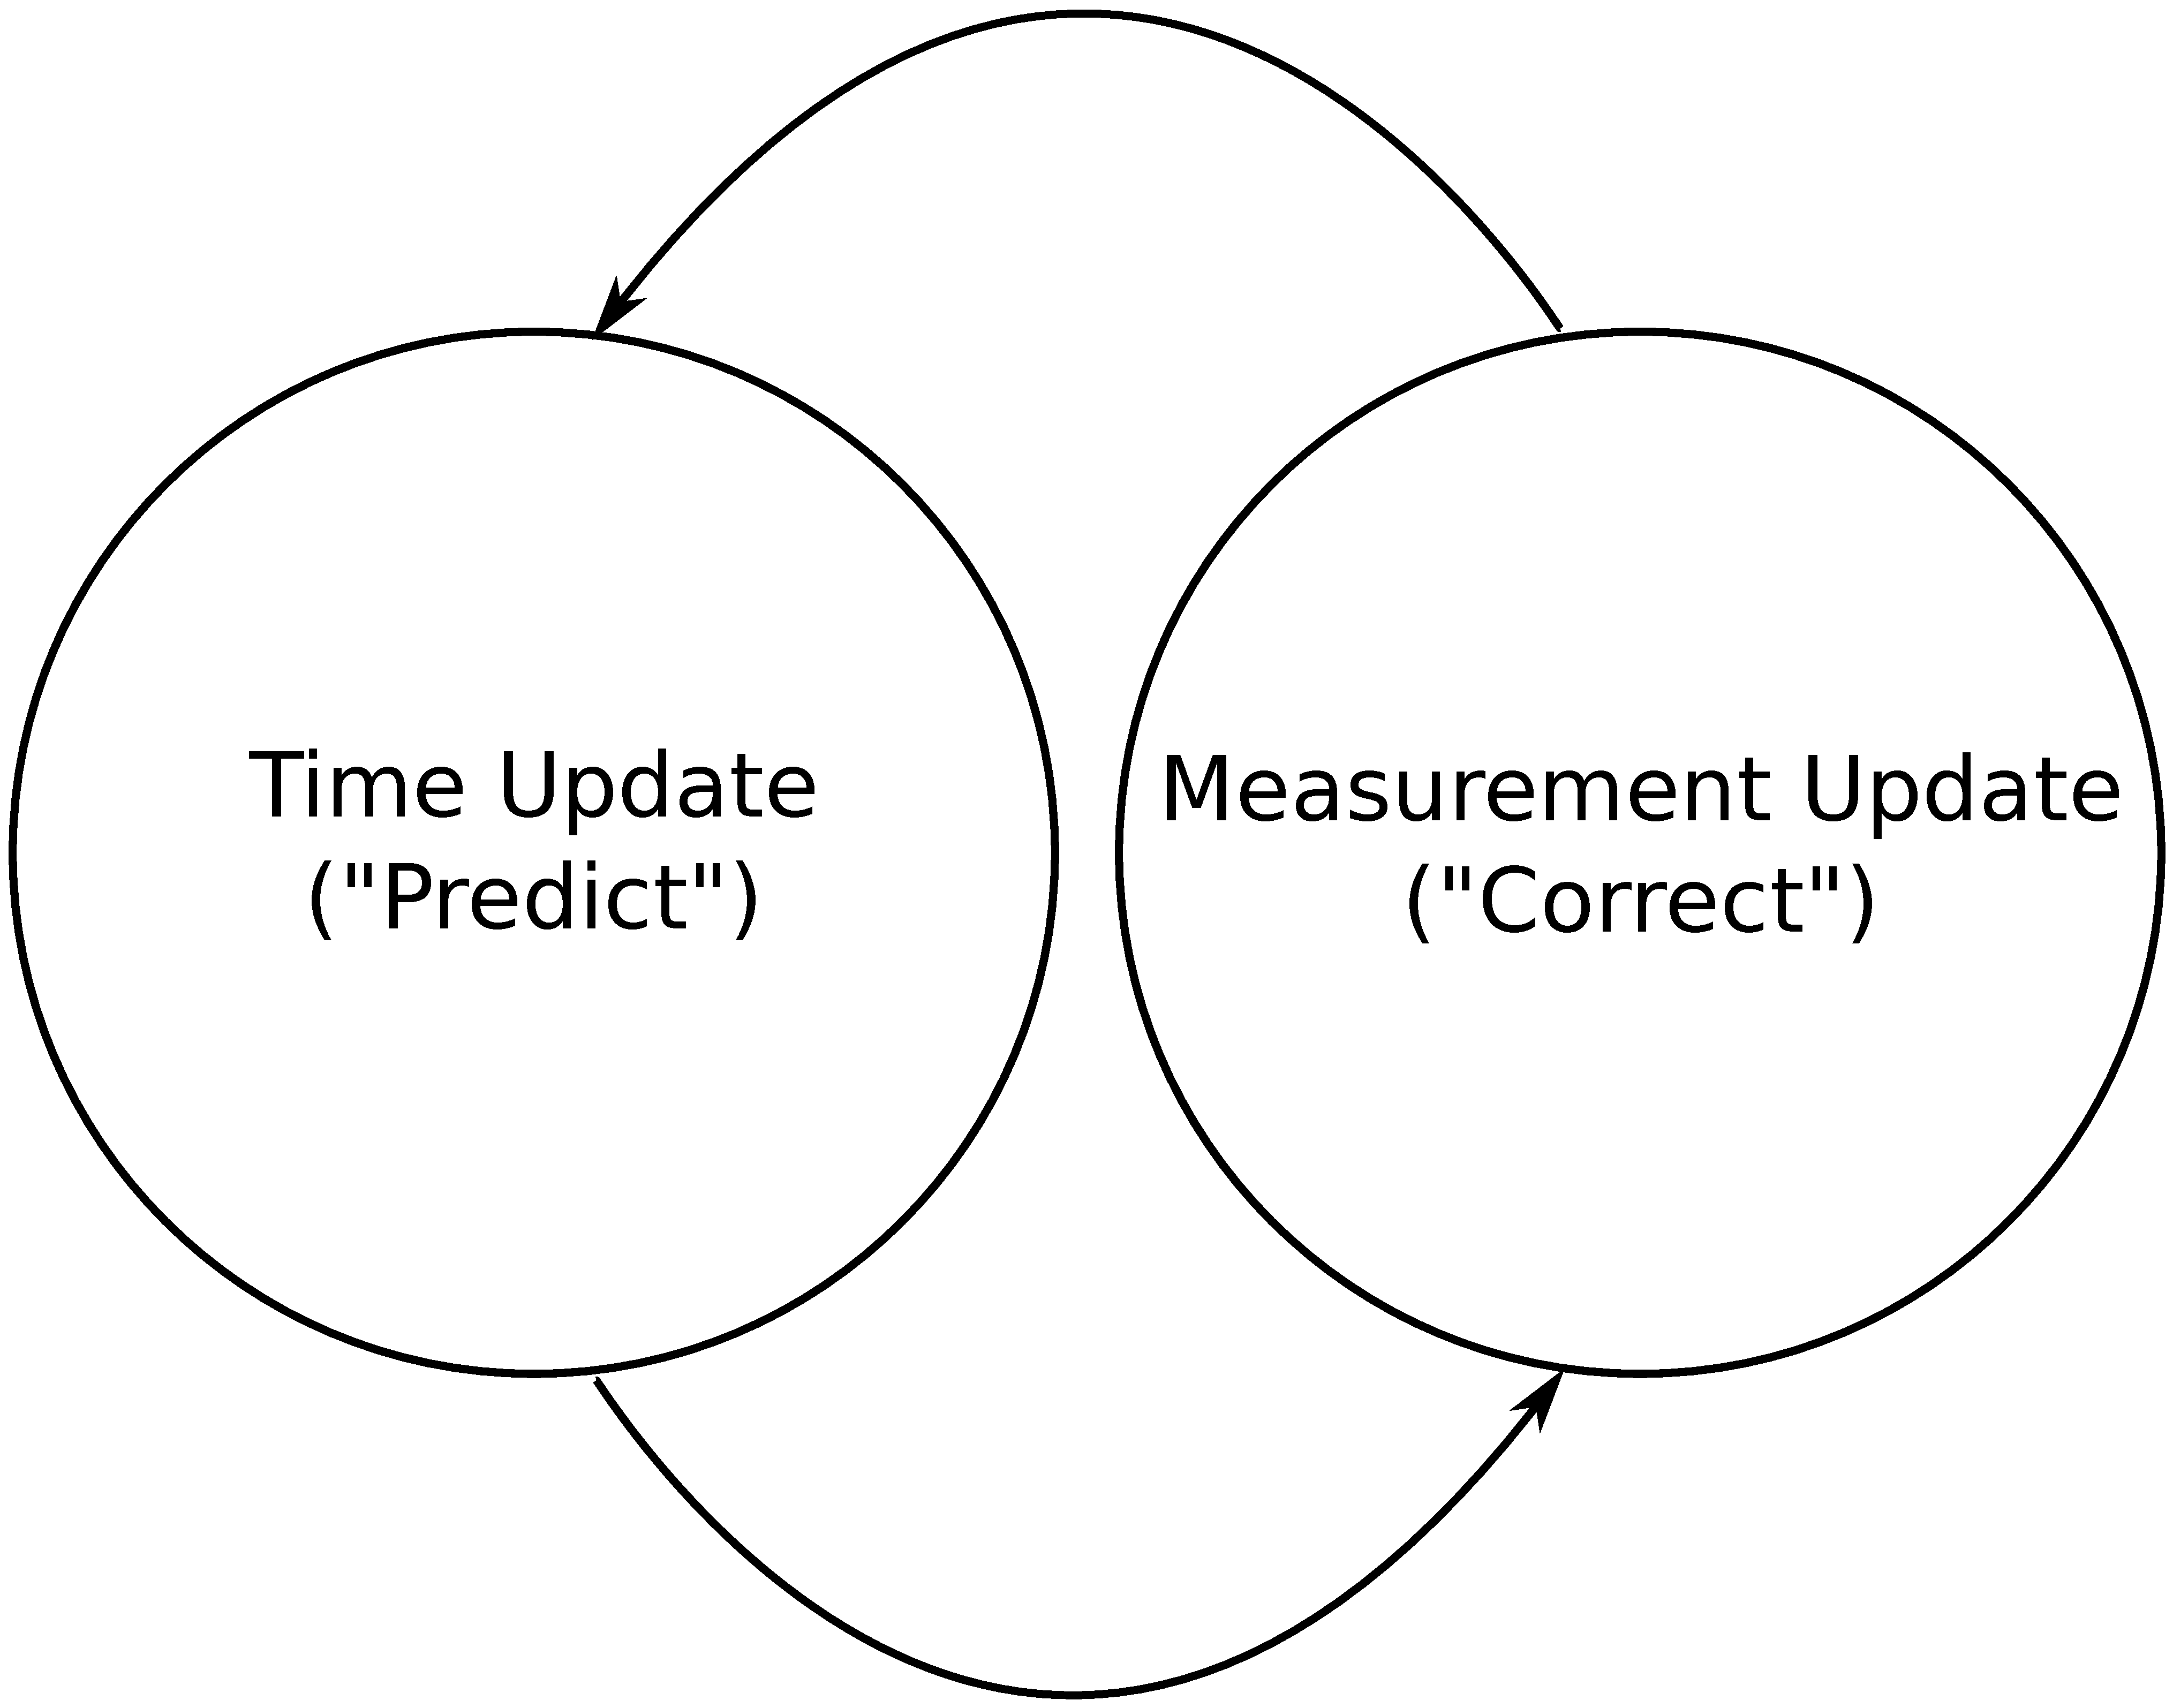
\includegraphics[width=0.5\linewidth]{kalman/fig/diagram-kalman.eps}
  \caption{Filtering process.}
\label{fig:diagram-kalman}
\end{figure}

One of its particularly useful features is the ability to combine together sensor measurements in mathematical form such that the solution is best possible estimate of the mean and the variance. 

Kalman filter uses three basic stages: prediction measurement and update. This would mean that the mean and the variance of the state are measureable. Prediction in case of moving vehicle is calculated based on previous vehicle location and dead reckoning.

Kalman gain determines the relationship between the importance of each previous estimation () and the current measurement (). Essentially - it expresses how much we trust in the measurement with respect to what we prediceted. According to the formula (), it is determined by matrices $Q$ and $R$ which represent process noise covariance and the measurement noise covariance (uncertainty), respectively. It takes values between 0 and 1 with 0 meaning that we use estimation only and give no importance to the measurement, and 1 that we consider direct measurement as the only important one.   

\section{Extended Kalman Filter (EKF)}

Real world models are rarely linear. The motiv for developing the Extended Kalman Filter is the adaptation of the linear Kalman Filter to dealing with nonlinear problems. However, it is possible that EKF significantly declines the performance quality \cite{julier96}. When making a prediction of state, observation or uncertainty of any of those for nonlinear systems, linearization can introduce errors. One example of such case is given in \cite{julier96}. The object follows the circular path. In such quite common case, the reason for failing in prediction is in linear approximations that EKF, by nature, uses when predicting the next state and its characteristics.

\section{Unscented Kalman Filter (UKF)}
Calculation-wise, the whole procedure is better than linearisation algorithm since there is no need for calculating the Jacobian, number of computations stays the same and it is easier to improvise with the algorithm by constraining or changing the samples \cite{julier96}.
\begin{algorithm}
\caption{UKF algorithm}
\label{alg:ukf}                   
%%%\begin{algorithmic}
%%%\INPUT state vector
%%%\OUTPUT feature vector \textit{fea}
%%%\FOR{$dist=0$ to $10$}
%%%\FORALL{$dir$ in \{0, 45, 90, 135\}}
%%%\STATE $glcm \leftarrow compute\ co-occurrence\ matrix\ for\ each\ pair\ of\ dist-dir$
%%%\STATE $normglcm \leftarrow normalize\ GLCM\ with\ the\ number\ of\ occurences$
%%%\STATE $harfea \leftarrow compute\ Haralick\ features$ \COMMENT{as in Appendix A}
%%%\STATE $fea \leftarrow [fea\ harfea]$ \COMMENT{store in feature vector}
%%%\ENDFOR
%%%\ENDFOR
%%%\end{algorithmic}
\end{algorithm}